\documentclass[11pt,oneside]{article}

\usepackage[a4paper,margin=25mm,headheight=15pt]{geometry}
\usepackage[T1]{fontenc}
\usepackage[utf8]{inputenc}
\IfFileExists{libertinus.sty}{\usepackage{libertinus}}{\usepackage{lmodern}}
\usepackage{microtype}
\usepackage{amsmath,amssymb,amsthm,mathtools,mathrsfs,bm}
\usepackage{booktabs,longtable,tabularx,array,multirow}
\usepackage{graphicx}
\usepackage{xcolor}
\usepackage{enumitem}
\usepackage{fancyhdr}
\usepackage{titlesec}
\usepackage{listings}
\usepackage{xurl}
\usepackage{hyperref}
\usepackage[nameinlink,noabbrev]{cleveref}
\usepackage[most]{tcolorbox}
\usepackage{caption}
\usepackage{float}

\definecolor{linkblue}{RGB}{25,75,135}
\definecolor{deepblue}{RGB}{20,54,94}
\definecolor{newgreen}{RGB}{28,105,70}
\definecolor{estgray}{RGB}{75,84,94}
\definecolor{conjorange}{RGB}{150,85,20}
\definecolor{shadegray}{RGB}{246,247,249}
\definecolor{rulegray}{RGB}{195,201,208}
\definecolor{lightblue}{RGB}{239,246,252}
\definecolor{lightgreen}{RGB}{239,249,244}
\definecolor{lightorange}{RGB}{253,246,237}

\hypersetup{
  colorlinks=true,
  linkcolor=linkblue,
  citecolor=linkblue,
  urlcolor=linkblue,
  pdftitle={Midpoint Transmutation, Dyadic Cardinal Reproduction, and Holonomic Obstructions},
  pdfauthor={Frontier report for the ProveIt FabiusFunction corpus},
  pdfsubject={Fabius function, inverse Fabius function, Rvachev up-function, Thue--Morse, q-calculus, Lambert W, Bell polynomials, Bernoulli polynomials, Strang--Fix, D-finite functions},
  pdfkeywords={Fabius function, Rvachev up-function, inverse Fabius, Thue-Morse, Lambert W, q-binomial, Bell polynomial, Bernoulli polynomial, Lagrange inversion, Richardson extrapolation, Strang-Fix, D-finite}
}

\pagestyle{fancy}
\fancyhf{}
\fancyhead[L]{\small Fabius--Rvachev frontier deductions}
\fancyhead[R]{\small\nouppercase{\leftmark}}
\fancyfoot[C]{\thepage}
\renewcommand{\headrulewidth}{0.4pt}

\titleformat{\section}{\Large\bfseries\color{deepblue}}{\thesection}{0.7em}{}
\titleformat{\subsection}{\large\bfseries}{\thesubsection}{0.7em}{}
\titleformat{\subsubsection}{\normalsize\bfseries}{\thesubsubsection}{0.7em}{}
\setcounter{secnumdepth}{3}
\setcounter{tocdepth}{2}
\setlist[itemize]{leftmargin=2em,itemsep=0.25em,topsep=0.4em}
\setlist[enumerate]{leftmargin=2.3em,itemsep=0.25em,topsep=0.4em}
\setlength{\emergencystretch}{3em}
\renewcommand{\arraystretch}{1.13}

\newtheorem{theorem}{Theorem}[section]
\newtheorem{proposition}[theorem]{Proposition}
\newtheorem{lemma}[theorem]{Lemma}
\newtheorem{corollary}[theorem]{Corollary}
\newtheorem{conjecture}[theorem]{Conjecture}
\theoremstyle{definition}
\newtheorem{definition}[theorem]{Definition}
\newtheorem{algorithm}[theorem]{Algorithm}
\newtheorem{example}[theorem]{Example}
\theoremstyle{remark}
\newtheorem{remark}[theorem]{Remark}
\newtheorem{warning}[theorem]{Warning}

\newtcolorbox{corpusdeductionbox}[1][]{
  breakable,
  colback=lightgreen,
  colframe=newgreen,
  fonttitle=\bfseries,
  title={Corpus-relative new deduction},
  #1
}
\newtcolorbox{establishedinputbox}[1][]{
  breakable,
  colback=shadegray,
  colframe=estgray,
  fonttitle=\bfseries,
  title={Established input},
  #1
}
\newtcolorbox{frontieropenbox}[1][]{
  breakable,
  colback=lightorange,
  colframe=conjorange,
  fonttitle=\bfseries,
  title={Open or conjectural direction},
  #1
}
\newtcolorbox{mainpointbox}[1][]{
  breakable,
  colback=lightblue,
  colframe=deepblue,
  fonttitle=\bfseries,
  title={Main point},
  #1
}

\lstdefinestyle{code}{
  basicstyle=\ttfamily\footnotesize,
  backgroundcolor=\color{shadegray},
  frame=single,
  rulecolor=\color{rulegray},
  columns=fullflexible,
  keepspaces=true,
  showstringspaces=false,
  breaklines=true,
  xleftmargin=0.7em,
  xrightmargin=0.7em,
  aboveskip=0.8em,
  belowskip=0.8em
}
\lstdefinestyle{manifest}{
  basicstyle=\ttfamily\scriptsize,
  backgroundcolor=\color{shadegray},
  frame=single,
  rulecolor=\color{rulegray},
  columns=fullflexible,
  keepspaces=true,
  showstringspaces=false,
  breaklines=true,
  xleftmargin=0.3em,
  xrightmargin=0.3em,
  aboveskip=0.5em,
  belowskip=0.5em
}

\newcommand{\R}{\mathbb R}
\newcommand{\C}{\mathbb C}
\newcommand{\N}{\mathbb N}
\newcommand{\Z}{\mathbb Z}
\newcommand{\Q}{\mathbb Q}
\newcommand{\Up}{\operatorname{up}}
\newcommand{\wt}{\operatorname{wt}_2}
\newcommand{\ord}{\operatorname{ord}}
\newcommand{\supp}{\operatorname{supp}}
\newcommand{\E}{\mathbb E}
\newcommand{\Var}{\operatorname{Var}}
\newcommand{\e}{\mathrm e}
\newcommand{\ii}{\mathrm i}
\newcommand{\dd}{\,\mathrm d}
\newcommand{\bigO}{\mathcal O}
\newcommand{\smallo}{o}
\newcommand{\D}{\mathrm D}
\newcommand{\repo}{\nolinkurl{Analysis/FabiusFunction/docs}}
\newcommand{\qbinom}[3]{\genfrac{[}{]}{0pt}{}{#1}{#2}_{#3}}
\newcommand{\qpoch}[2]{(#1;#2)}
\newcommand{\Dyad}{\mathbb D_2}
\newcommand{\Acard}{\mathcal A}
\newcommand{\M}{\mathcal M}
\DeclareMathOperator{\sinc}{sinc}
\DeclareMathOperator{\sgn}{sgn}

\title{\bfseries Midpoint Transmutation, Dyadic Cardinal Reproduction,\
and Holonomic Obstructions\\[0.4em]
\large New deductions around the Fabius function, its inverse, Rvachev's up-function,\
Thue--Morse cancellation, Lambert--W asymptotics, and q-scale algebra}
\author{A corpus-relative frontier report for Vladimir Reshetnikov's \texttt{ProveIt} repository}
\date{Repository snapshot audited: 27 August 2026}

\begin{document}
\maketitle

\begin{abstract}
A recursive audit of the fifty-seven \LaTeX{} sources under \repo\ reveals a mature body of work on exact dyadic arithmetic, Thue--Morse prefix sums, q-binomial coefficient extraction, infinite sinc and cosine products, sharp Fourier and endpoint asymptotics, lower-branch Lambert--W coordinates, Bell-polynomial saddle algebra, Lagrange interpolation, and Richardson acceleration.  This report deliberately avoids reproducing those developments.  Instead it develops three complementary branches that were not found in the audited corpus.

First, an exact identity transports the left-endpoint germ of the Fabius function to its midpoint:
\[
 F\!\left(\frac12\pm h\right)=\frac12\pm2h\mp F(h),\qquad 0\le h\le\frac12.
\]
It follows that the Taylor jet of $F$ at $1/2$ is exactly affine although $F$ is not analytic there.  For the inverse $I=F^{-1}$, writing $z=\delta/2$ and
$h=I(1/2+\delta)-1/2$ gives the exact fixed-point equation
$h=z+F(h)/2$.  The inverse defect $E(\delta)=h-z$ is flat to every order and satisfies
$E(\delta)\sim F(\delta/2)/2$.  Therefore the repository's complete lower-Lambert endpoint expansion transfers, coefficient for coefficient, to the first nontrivial correction of the inverse at its midpoint.  A finite, rigorous Lagrange--Bell jet with an integral remainder is also obtained.

Second, dyadic dilations $U_r(x)=2^{-r}\Up(2^{-r}x)$ form a cardinal reproduction ladder.  Their Fourier transforms have zeros of order at least $r+1$ at every nonzero integer, a property whose finite block is exactly the Prouhet cancellation of a length-$2^{r+1}$ signed Thue--Morse word.  Consequently
\[
 \sum_{k\in\Z}(x-k)^jU_r(x-k)=\int_{\R}y^jU_r(y)\dd y,
 \qquad 0\le j\le r.
\]
Reciprocal-moment Appell polynomials $\Acard_n^{[r]}$ then give finite exact formulas
$\sum_k\Acard_n^{[r]}(k)U_r(x-k)=x^n$ for $n\le r$.  Their coefficients are explicit complete Bell polynomials in Bernoulli cumulants; their dyadic scale transport is governed by the Bernoulli-polynomial values $B_n(1/2)$; and, because $\Acard_n(x;Q)$ is polynomial in $Q=4^r$, the scale sequence obeys exact q-binomial finite-difference closures at $q=1/4$.

Third, two independent obstructions exclude holonomicity.  The midpoint identity propagates nonanalyticity backward through the dyadic tent map, proving that $F$ is nonanalytic at every dyadic rational; the same mechanism gives dense nonanalytic sets for $F^{-1}$ and $\Up$.  Hence none is locally D-finite on any open interval.  Independently, the unbounded multiplicities
$\ord_m\widehat\Up=1+\nu_2(|m|)$ rule out a polynomial-coefficient differential equation for the entire Fourier transform.  This implies non-D-finiteness of the moment generating functions, non-P-recursiveness of the moment sequences, and non-P-recursiveness of every fixed-$x$ Appell coefficient sequence.  Symbolic and high-precision numerical experiments accompany the proofs, and the fully commented Python program is included in the archive.
\end{abstract}

\begin{tcolorbox}[colback=lightorange,colframe=conjorange,title=Priority and novelty disclaimer,fonttitle=\bfseries]
The word \emph{new} in this report means \emph{not found in the audited repository snapshot}.  It is not a claim of global historical priority.  In particular, general Strang--Fix theory and nonstationary multiresolution analysis based on the up-function already exist in the approximation-theory literature~\cite{strangFix,dynRon,liShen}.  The corpus-relative contribution here is the explicit dilation-indexed cardinal ladder, its Prouhet factorization, the Bernoulli--Bell coefficient formulas, and their exact q-scale closure, together with the midpoint/inverse and holonomic deductions.
\end{tcolorbox}

\tableofcontents
\newpage

\section{Corpus audit and non-duplication protocol}
\label{sec:audit}

\subsection{What was audited}
The recursive tree under \repo\ contains twenty-five living or current-tree TeX sources and thirty-two frozen archive sources~\cite{proveit,primary,frontier,atlas}.  The living group includes the primary exposition, the non-elementarity article, the Lean walkthrough, the mathematical glossary, the consolidated non-formalized frontier, the living Thue--Morse Formula Atlas, twelve Fourier-decay drafts or audits, and seven transcribed research papers.  The archive preserves early notes, parallel primary expositions, supplements, q-calculus articles, walkthroughs, glossaries, per-topic frontier dossiers, and three predecessor Atlas consolidations.

The archive ledger explains that current-head byte-identical copies were pruned and that the remaining documents are frozen historical versions.  Accordingly, this audit used three levels of comparison:
\begin{enumerate}
\item direct reading of the living canonical exposition, consolidated frontier, Atlas, distinct Fourier-decay documents, and paper transcriptions;
\item topic-by-topic comparison with every archived entry and its stated scope;
\item targeted full-text searches for the candidate branches developed below, including close variants of ``Strang--Fix'', ``polynomial reproduction'', ``inverse-moment Appell'', ``D-finite'', ``holonomic'', ``P-recursive'', and the continuous midpoint identity of \cref{thm:midpoint-transmutation}.
\end{enumerate}
The complete path inventory is reproduced in \cref{app:manifest} and included as a separate machine-readable file, \texttt{corpus\_manifest.txt}.

\subsection{The overlap map}
The repository already treats the following subjects in substantial depth:
\begin{itemize}
\item exact rational values $F(a/2^n)$, triangular recurrences, composition sums, q-Pochhammer symbols, Gaussian binomials, and coefficient extraction;
\item Thue--Morse product identities, Prouhet cancellation, iterated prefix sums, finite convolution laws, and sharp convergence rates;
\item the sinc and cosine products for $\widehat\Up$, Fourier decay, zero sets, and refined log-periodic asymptotics;
\item lower-branch Lambert--W coordinates for $F(x)$ as $x\downarrow0$, periodic saddle jets, and all-orders Bell-polynomial contraction formulas;
\item exact and asymptotic Lagrange interpolation, q-interpolation, and Richardson-type acceleration at dyadic scales;
\item repeated-integration and finite-box-spline approximants to $\Up$, including exact tail replacement and quantitative error decompositions;
\item inverse-function basics, including $I(1/2)=1/2$, $I'(1/2)=1/2$, and $I''(1/2)=0$.
\end{itemize}
These are inputs, not claimed results of this report.  In particular, the q-binomial weights in \cref{sec:qscale} are familiar from the repository's q-Richardson work; what is new here is that they annihilate a newly constructed, exact polynomial-in-scale Appell family rather than an asymptotic error model.

\begin{mainpointbox}[title=Three principal corpus gaps]
The audit did not reveal a treatment of:
\begin{enumerate}
\item the exact continuous midpoint--endpoint identity, its all-orders inverse consequence, or the transfer of endpoint Lambert--W asymptotics to the inverse midpoint defect;
\item a Strang--Fix/cardinal polynomial reproduction ladder for the dyadically dilated up-function, with reciprocal-moment Appell correctors and Bernoulli--Bell scale algebra;
\item D-finite and P-recursive obstructions derived simultaneously from dense dyadic nonanalyticity and unbounded Fourier-zero multiplicity.
\end{enumerate}
\end{mainpointbox}

\subsection{Status labels used below}
Gray boxes mark established inputs from the repository or standard literature.  Green boxes mark deductions that appear new relative to the audited corpus.  Orange boxes contain conjectures, extensions, or research programs whose proofs are not supplied.  Numerical evidence is never used in place of proof.

\section{Established framework and notation}
\label{sec:framework}

\subsection{The three functions}
Let $F:\R\to[0,1]$ be the bounded Fabius distribution function, normalized by
\[
 F(x)=0\quad(x\le0),\qquad F(x)=1\quad(x\ge1),
\]
and, on $[0,1]$, by
\begin{equation}
 F'(x)=2F(2x)\quad\left(0\le x\le\frac12\right),
 \qquad F(1-x)=1-F(x).
 \label{eq:fabius-basic}
\end{equation}
It is $C^\infty$, strictly increasing on $(0,1)$, and flat at both endpoints.  Let $I=F^{-1}:(0,1)\to(0,1)$ be its ordinary inverse.

Rvachev's even up-function $U=\Up$ is supported on $[-1,1]$, integrates to one, and satisfies~\cite{ariasUp,ariasArithmetic}
\begin{equation}
 U(x)=F(1-|x|),\qquad |x|\le1.
 \label{eq:up-fabius}
\end{equation}
Equivalently, $F(x)=U(x-1)$ on $[0,1]$.

It is useful to write the symmetric tent map
\begin{equation}
 \tau(x)=
 \begin{cases}
  2x,&0\le x\le\frac12,\\
  2-2x,&\frac12\le x\le1.
 \end{cases}
 \label{eq:tent}
\end{equation}
Differentiating the symmetry in \eqref{eq:fabius-basic} gives the global interior identity
\begin{equation}
 F'(x)=2F(\tau(x)),\qquad 0<x<1.
 \label{eq:tent-derivative}
\end{equation}

\subsection{Probability, Fourier, and moments}
Use the Fourier convention
\begin{equation}
 \widehat f(\xi)=\int_{\R}f(x)\e^{-2\pi\ii x\xi}\dd x.
 \label{eq:fourier-convention}
\end{equation}
Let $V_n$ be independent uniform variables on
$[-2^{-n-1},2^{-n-1}]$.  Then
\begin{equation}
 X=\sum_{n=0}^{\infty}V_n
 \label{eq:random-series}
\end{equation}
converges absolutely and has density $U$.  Therefore
\begin{align}
 \widehat U(\xi)
 &=\prod_{n=0}^{\infty}
   \frac{\sin(\pi\xi/2^n)}{\pi\xi/2^n}
  =\prod_{n=0}^{\infty}\sinc\!\left(\frac{\pi\xi}{2^n}\right),
 \label{eq:sinc-product}\\
 &=\prod_{m=1}^{\infty}
   \left(\cos\frac{\pi\xi}{2^m}\right)^m.
 \label{eq:cos-product}
\end{align}
The moment generating function is the entire even function
\begin{equation}
 \M_0(t)=\E\e^{tX}
 =\prod_{n=0}^{\infty}
   \frac{\sinh(t/2^{n+1})}{t/2^{n+1}}
 =\widehat U\!\left(\frac{\ii t}{2\pi}\right).
 \label{eq:mgf}
\end{equation}

\subsection{The imported endpoint coordinate}
Put $L=\log2$ and define the lower-Lambert coordinate~\cite{corless,frontier}
\begin{equation}
 \lambda(x)=-\frac1L W_{-1}(-Lx),
 \qquad \lambda(x)2^{-\lambda(x)}=x.
 \label{eq:lambda}
\end{equation}
The repository develops a complete endpoint expansion whose first structural layer has the form
\begin{equation}
 \log F(x)
 =-\frac L2\lambda^2
  +\left(1+\frac L2\right)\lambda
  -\frac12\log\lambda
  +C_F+\Psi(\lambda)
  +\sum_{j=1}^{N-1}\frac{A_j(\lambda)}{\lambda^j}
  +\bigO(\lambda^{-N}).
 \label{eq:imported-endpoint}
\end{equation}
Here $\lambda=\lambda(x)$; $\Psi$ and the higher coefficient functions encode the dyadic phase and are periodic in the normalization of the frontier documents.  The precise normalization of $C_F$, $\Psi$, and $A_j$ is left to those sources.  The point of \cref{sec:inverse-midpoint} is that every term in \eqref{eq:imported-endpoint} transfers unchanged to an inverse-function defect after replacing $x$ by $\delta/2$ and subtracting $\log2$.

\begin{establishedinputbox}
Nothing in \cref{sec:framework} is claimed as new.  These identities fix conventions and isolate the exact inputs used later.
\end{establishedinputbox}

\section{An exact midpoint--endpoint transmutation}
\label{sec:midpoint}

\begin{theorem}[Midpoint--endpoint transmutation]
\label{thm:midpoint-transmutation}
For every $0\le h\le1/2$,
\begin{align}
 F\!\left(\frac12+h\right)&=\frac12+2h-F(h),
 \label{eq:midpoint-plus}\\
 F\!\left(\frac12-h\right)&=\frac12-2h+F(h).
 \label{eq:midpoint-minus}
\end{align}
\end{theorem}

\begin{proof}
Integrating the differential equation in \eqref{eq:fabius-basic} gives
\begin{equation}
 F(h)=\int_0^h2F(2t)\dd t=\int_0^{2h}F(u)\dd u.
 \label{eq:F-integral}
\end{equation}
On the other hand,
\begin{align*}
 F\!\left(\frac12\right)-F\!\left(\frac12-h\right)
 &=\int_{1/2-h}^{1/2}2F(2t)\dd t\\
 &=\int_{1-2h}^{1}F(u)\dd u\\
 &=\int_0^{2h}F(1-v)\dd v\\
 &=2h-\int_0^{2h}F(v)\dd v
 =2h-F(h).
\end{align*}
Since $F(1/2)=1/2$, this proves \eqref{eq:midpoint-minus}; symmetry gives \eqref{eq:midpoint-plus}.
\end{proof}

\begin{corpusdeductionbox}
The theorem says that the entire nontrivial midpoint germ is exactly the endpoint germ with a sign change after removal of the affine tangent.  This is a functional identity, not the finite-approximant midpoint formula already present in the archived Thue--Morse convergence report.
\end{corpusdeductionbox}

\subsection{The complete midpoint jet}
\begin{corollary}[Affine Taylor jet and nonanalyticity]
\label{cor:midpoint-jet}
The derivatives of $F$ at the midpoint are
\begin{equation}
 F\!\left(\frac12\right)=\frac12,
 \qquad F'\!\left(\frac12\right)=2,
 \qquad F^{(m)}\!\left(\frac12\right)=0\quad(m\ge2).
 \label{eq:midpoint-jet}
\end{equation}
Nevertheless, $F$ is not real analytic at $1/2$.
\end{corollary}

\begin{proof}
The endpoint flatness $F^{(m)}(0)=0$ for every $m\ge0$ and \eqref{eq:midpoint-plus} give \eqref{eq:midpoint-jet}.  If $F$ were analytic at $1/2$, its Taylor series would force
$F(1/2+h)=1/2+2h$ for all sufficiently small $h$, contradicting $F(h)>0$ in \eqref{eq:midpoint-plus}.
\end{proof}

Thus the flat endpoint term is invisible to every finite-order midpoint Taylor method.  In numerical analysis language, it is a beyond-all-orders defect; in quasianalyticity language, the midpoint germ lies outside every class in which the Taylor map is injective.

\subsection{Central integral identities}
The transmutation has immediate exact integral consequences.  For $0\le a\le1/2$,
\begin{align}
 \int_{1/2-a}^{1/2+a}F(x)\dd x&=a,
 \label{eq:central-mass}\\
 \int_0^a\left[F\!\left(\frac12+h\right)-\frac12-2h\right]\dd h
 &=-\int_0^aF(h)\dd h.
 \label{eq:central-defect-integral}
\end{align}
The first is also a direct consequence of symmetry, while the second identifies the exact signed central curvature budget with the endpoint mass.  Repeated integration of \eqref{eq:midpoint-plus} similarly transports all endpoint primitives to the midpoint.

\section{The inverse midpoint defect and its Lambert--W transfer}
\label{sec:inverse-midpoint}

\subsection{An exact fixed-point equation}
Let $I=F^{-1}$.  For $0\le\delta<1/2$ define
\begin{equation}
 h(\delta)=I\!\left(\frac12+\delta\right)-\frac12,
 \qquad z=\frac\delta2,
 \qquad E(\delta)=h(\delta)-z.
 \label{eq:inverse-definitions}
\end{equation}
Since $F(1/2+h)=1/2+\delta$, \cref{thm:midpoint-transmutation} gives the exact equation
\begin{equation}
 \delta=2h-F(h),
 \qquad
 h=z+\frac12F(h),
 \qquad
 E(\delta)=\frac12F(z+E(\delta)).
 \label{eq:inverse-fixed-point}
\end{equation}
For negative $\delta$, inverse symmetry gives
\begin{equation}
 I\!\left(\frac12+\delta\right)
 =\frac12+\frac\delta2+\sgn(\delta)E(|\delta|).
 \label{eq:inverse-odd-defect}
\end{equation}

\begin{theorem}[All-orders inverse midpoint flatness]
\label{thm:inverse-flatness}
The inverse $I$ is $C^\infty$ on $(0,1)$ and
\begin{equation}
 I'\!\left(\frac12\right)=\frac12,
 \qquad I^{(m)}\!\left(\frac12\right)=0\quad(m\ge2).
 \label{eq:inverse-jet}
\end{equation}
More strongly, for every $N\ge1$,
\begin{equation}
 E(\delta)=\bigO(\delta^N)\qquad(\delta\downarrow0).
 \label{eq:E-flat}
\end{equation}
The inverse is not analytic at $1/2$.
\end{theorem}

\begin{proof}
The inverse is smooth because $F'(x)>0$ for $0<x<1$.  From \eqref{eq:inverse-fixed-point}, $h\to0$ with $\delta$ and
\[
 \frac\delta h=2-\frac{F(h)}h\longrightarrow2
\]
because $F$ is flat at zero.  Hence $h\sim\delta/2$.  The same equation yields
$E=F(h)/2=\bigO(h^N)=\bigO(\delta^N)$ for every $N$.  Equation \eqref{eq:inverse-odd-defect} then gives the complete jet \eqref{eq:inverse-jet}.  Analyticity would force $I(1/2+\delta)=1/2+\delta/2$ locally, contradicting $E(\delta)>0$.
\end{proof}

\subsection{Certified monotone inversion}
The fixed-point equation is not merely asymptotic; it gives a certified algorithm.

\begin{proposition}[Two-sided fixed-point iteration]
\label{prop:certified-iteration}
Fix $0<\delta<1/2$, put $z=\delta/2$, and define
\[
 T_z(t)=z+\frac12F(t),
 \qquad b=z+\frac14.
\]
Then $T_z$ maps $[z,b]$ into itself and is a contraction there with constant
\begin{equation}
 q_\delta=F\!\left(\frac12+\delta\right)<1.
 \label{eq:qdelta}
\end{equation}
The lower iteration $\ell_0=z$, $\ell_{n+1}=T_z(\ell_n)$ increases to $h$, while the upper iteration $u_0=b$, $u_{n+1}=T_z(u_n)$ decreases to $h$.  Moreover,
\begin{equation}
 0\le h-\ell_n\le\frac{q_\delta^n}{1-q_\delta}(\ell_1-\ell_0),
 \qquad
 0\le u_n-h\le\frac{q_\delta^n}{1-q_\delta}(u_0-u_1).
 \label{eq:iteration-errors}
\end{equation}
\end{proposition}

\begin{proof}
For $t\in[z,b]\subset[0,1/2)$, monotonicity gives $0\le F(t)\le1/2$, hence
$z\le T_z(t)\le z+1/4=b$.  Also
\[
 T_z'(t)=\frac12F'(t)=F(2t)
 \le F(2b)=F\!\left(\frac12+\delta\right)=q_\delta<1.
\]
The contraction theorem and monotonicity prove the assertions; the displayed estimates are the standard geometric a posteriori bounds.
\end{proof}

This gives a simple inverse evaluator requiring only forward evaluations of $F$, with no numerical differentiation and a rigorous enclosure at every step.

\subsection{Sharp leading comparison}
\begin{proposition}[Endpoint proxy for the inverse defect]
\label{prop:inverse-proxy}
For each $0<\delta<1/2$ there exists $\xi_\delta\in(z,h)$ such that
\begin{equation}
 E(\delta)=\frac{F(z)}{2-F'(\xi_\delta)}
 =\frac{F(z)}2\frac1{1-F'(\xi_\delta)/2}.
 \label{eq:exact-proxy}
\end{equation}
Consequently
\begin{equation}
 E(\delta)\sim\frac12F\!\left(\frac\delta2\right),
 \qquad \delta\downarrow0,
 \label{eq:inverse-leading}
\end{equation}
and
\begin{equation}
 \log E(\delta)
 =\log F\!\left(\frac\delta2\right)-\log2
  +\bigO(F'(h(\delta))).
 \label{eq:log-proxy}
\end{equation}
\end{proposition}

\begin{proof}
Apply the mean-value theorem to $F(z+E)-F(z)$ in \eqref{eq:inverse-fixed-point}:
\[
 2E=F(z)+F'(\xi_\delta)E.
\]
This is \eqref{eq:exact-proxy}.  Since $\xi_\delta\to0$ and $F'(0)=0$, the ratio in \eqref{eq:inverse-leading} tends to one.  Taking logarithms and using $-\log(1-u)=\bigO(u)$ proves \eqref{eq:log-proxy}.
\end{proof}

\begin{corpusdeductionbox}[title=Lambert--W transfer theorem]
Let $z=\delta/2$ and $\lambda=\lambda(z)$ as in \eqref{eq:lambda}.  The correction term in \eqref{eq:log-proxy} is smaller than every algebraic power of $1/\lambda$.  Therefore any complete endpoint expansion of the form \eqref{eq:imported-endpoint} transfers term by term:
\begin{align}
 \log E(\delta)
 &=-\frac L2\lambda^2
  +\left(1+\frac L2\right)\lambda
  -\frac12\log\lambda
  +C_F+\Psi(\lambda)-\log2
 \notag\\
 &\quad+\sum_{j=1}^{N-1}\frac{A_j(\lambda)}{\lambda^j}
  +\bigO(\lambda^{-N}).
 \label{eq:inverse-lambert-transfer}
\end{align}
Thus the inverse midpoint defect has the same dyadic phase, the same Bell-polynomial saddle coefficients, and the same lower-Lambert coordinate as the endpoint function, evaluated at half the ordinate displacement.
\end{corpusdeductionbox}

\subsection{A rigorous Lagrange--Bell jet}
Set $\phi=F/2$ and introduce a coupling parameter $\varepsilon$:
\begin{equation}
 h_\varepsilon=z+\varepsilon\phi(h_\varepsilon),
 \qquad 0\le\varepsilon\le1.
 \label{eq:coupled-fixed-point}
\end{equation}
For fixed $z\in(0,1/4)$, the implicit-function denominator
$1-\varepsilon\phi'(h_\varepsilon)$ stays positive, so $h_\varepsilon$ is $C^\infty$ in $\varepsilon$.

\begin{theorem}[Finite Lagrange--Bell expansion with exact remainder]
\label{thm:lagrange-bell}
For every $N\ge1$,
\begin{equation}
 h_1=z+\sum_{n=1}^{N}\frac1{n!}
 \D_z^{n-1}\!\left[\phi(z)^n\right]+R_N(z),
 \label{eq:lagrange-finite}
\end{equation}
where
\begin{equation}
 R_N(z)=\frac1{N!}\int_0^1(1-\varepsilon)^N
 \frac{\partial^{N+1}h_\varepsilon}{\partial\varepsilon^{N+1}}\dd\varepsilon.
 \label{eq:lagrange-remainder}
\end{equation}
Moreover,
\begin{equation}
 \D^{n-1}(\phi^n)
 =\sum_{k=0}^{n-1}(n)_k\phi^{n-k}
 B_{n-1,k}(\phi',\phi'',\ldots),
 \label{eq:partial-bell}
\end{equation}
where $B_{m,k}$ is the partial exponential Bell polynomial and $(n)_k$ is a falling factorial.
\end{theorem}

\begin{proof}
The Lagrange--Buerhmann coefficient identity
\[
 \left.\frac{\partial^n h_\varepsilon}{\partial\varepsilon^n}\right|_{\varepsilon=0}
 =\D_z^{n-1}[\phi(z)^n]
\]
follows by formal differentiation of \eqref{eq:coupled-fixed-point}; because only a finite jet is asserted, $C^\infty$ regularity suffices and no analyticity of $F$ is needed.  Taylor's theorem in $\varepsilon$ with integral remainder gives \eqref{eq:lagrange-finite}--\eqref{eq:lagrange-remainder}.  Formula \eqref{eq:partial-bell} is Fa\`a di Bruno's formula applied to the power map $u\mapsto u^n$; see also the standard Bell-polynomial and umbral treatments~\cite{comtet,roman}.
\end{proof}

The first four correction layers, evaluated formally at $\varepsilon=1$, are
\begin{align}
 E
={}&\frac F2+\frac{FF'}4
 +\frac{F(F')^2}{8}+\frac{F^2F''}{16}
 \notag\\
 &+\frac{F(F')^3}{16}
  +\frac{3F^2F'F''}{32}
  +\frac{F^3F'''}{96}+\cdots,
 \label{eq:inverse-bell-first}
\end{align}
where every $F$ and derivative is evaluated at $z=\delta/2$.  Equation \eqref{eq:lagrange-finite}, rather than the ellipsis, is the rigorous statement.  Whether the full coupling series converges at $\varepsilon=1$ uniformly as $z\downarrow0$ is left open.

\section{Thue--Morse blocks and the dyadic zero architecture}
\label{sec:zero-architecture}

\subsection{Box convolutions}
For $a>0$ let
\begin{equation}
 b_a(x)=\frac1{2a}\mathbf1_{[-a,a]}(x),
 \qquad \widehat b_a(\xi)=\frac{\sin(2\pi a\xi)}{2\pi a\xi}.
 \label{eq:box}
\end{equation}
Then
\begin{equation}
 U=*_{n=0}^{\infty}b_{2^{-n-1}}.
 \label{eq:up-box-convolution}
\end{equation}
For $r\ge0$ define the normalized dilation
\begin{equation}
 U_r(x)=2^{-r}U(2^{-r}x),
 \qquad \supp U_r=[-2^r,2^r],
 \qquad \widehat U_r(\xi)=\widehat U(2^r\xi).
 \label{eq:Ur}
\end{equation}
Its first $r+1$ box factors form
\begin{equation}
 B_r=*_{j=0}^{r}b_{2^{r-j-1}}.
 \label{eq:Br}
\end{equation}

\begin{proposition}[Distributional Thue--Morse derivative]
\label{prop:tm-derivative}
In the sense of compactly supported distributions,
\begin{equation}
 \D^{r+1}B_r
 =2^{-r(r+1)/2}
 \sum_{n=0}^{2^{r+1}-1}
 (-1)^{\wt(n)}
 \delta_{\,n-(2^{r+1}-1)/2}.
 \label{eq:tm-derivative}
\end{equation}
\end{proposition}

\begin{proof}
Since
$\D b_a=(\delta_{-a}-\delta_a)/(2a)$, convolving the $r+1$ derivatives produces one atom for every binary choice of endpoints.  If the chosen positive endpoints have binary indicator $n$, their signs multiply to $(-1)^{\wt(n)}$, their location is
\[
 \sum_{j=0}^{r}(2\varepsilon_j-1)2^{r-j-1}
 =n-\frac{2^{r+1}-1}{2},
\]
and the product of normalizing factors is
$\prod_{j=0}^{r}2^{-(r-j)}=2^{-r(r+1)/2}$.
\end{proof}

The finite exponential sum in \eqref{eq:tm-derivative} has a zero of order $r+1$ at every integer frequency, the classical Prouhet cancellation encoded by the Thue--Morse word~\cite{prouhet,alloucheShallit}.  Indeed, after translation by an integer frequency, its Taylor coefficients through order $r$ are the Prouhet sums
\begin{equation}
 \sum_{n=0}^{2^{r+1}-1}(-1)^{\wt(n)}n^j=0,
 \qquad 0\le j\le r.
 \label{eq:prouhet}
\end{equation}
Thus the universal part of the integer zero multiplicity is literally the moment cancellation of one finite Thue--Morse block.

\subsection{Exact integer multiplicities}
\begin{proposition}[Dyadic zero multiplicity]
\label{prop:zero-multiplicity}
For every nonzero integer $m$,
\begin{equation}
 \ord_m\widehat U=1+\nu_2(|m|).
 \label{eq:zero-multiplicity}
\end{equation}
Consequently, for every nonzero $\ell\in\Z$,
\begin{equation}
 \ord_\ell\widehat U_r=r+1+\nu_2(|\ell|).
 \label{eq:scaled-zero-multiplicity}
\end{equation}
\end{proposition}

\begin{proof}
In \eqref{eq:sinc-product}, the factor indexed by $n$ vanishes at an integer $m$ exactly when $2^n$ divides $m$.  These zeros are simple, and all remaining factors are nonzero there, proving \eqref{eq:zero-multiplicity}.  Apply it to $2^r\ell$ to obtain \eqref{eq:scaled-zero-multiplicity}.
\end{proof}

\begin{figure}[H]
\centering
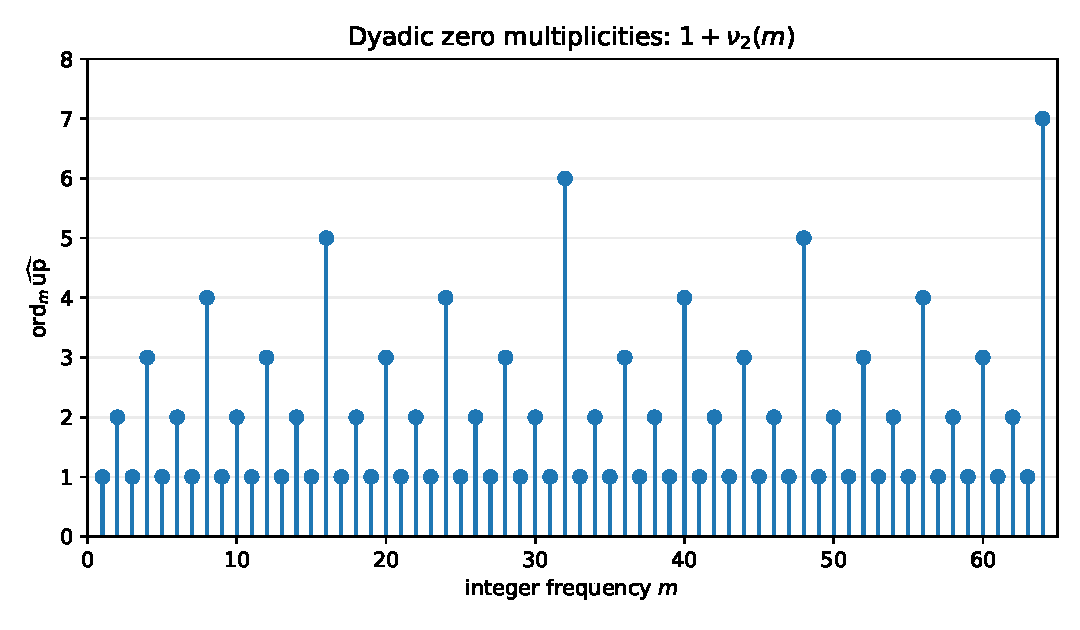
\includegraphics[width=0.92\textwidth]{figures/zero_multiplicity_ladder.pdf}
\caption{The exact multiplicities $1+\nu_2(m)$ for $1\le m\le64$.  The unbounded spikes at powers of two later obstruct D-finiteness of the entire Fourier transform.}
\label{fig:zero-multiplicity}
\end{figure}

\begin{remark}
The multiplicity formula is not used as a novelty claim by itself.  Its role here is structural: the first $r+1$ units of multiplicity are explained by the Prouhet block \eqref{eq:tm-derivative}, while the remaining $\nu_2(\ell)$ units come from the infinite tail.  This split is precisely what drives the cardinal reproduction order in the next section.
\end{remark}

\section{A dyadic cardinal reproduction ladder}
\label{sec:cardinal}

\subsection{Strang--Fix vanishing at every scale}
Equation \eqref{eq:scaled-zero-multiplicity} implies
\begin{equation}
 \widehat U_r^{(j)}(\ell)=0,
 \qquad \ell\in\Z\setminus\{0\},\quad 0\le j\le r.
 \label{eq:strang-fix}
\end{equation}
This is the one-dimensional Strang--Fix condition of order $r+1$ on the unit lattice.  General approximation theory already connects such vanishing to polynomial reproduction~\cite{strangFix,dynRon,liShen}.  The following exact formulas specialize that principle to the up-function and keep track of all moment corrections.

\begin{theorem}[Moment periodization]
\label{thm:moment-periodization}
Let
\begin{equation}
 \mu_j^{[r]}=\int_{\R}y^jU_r(y)\dd y.
 \label{eq:scaled-moments}
\end{equation}
For every $r\ge0$, every $0\le j\le r$, and every $x\in\R$,
\begin{equation}
 \sum_{k\in\Z}(x-k)^jU_r(x-k)=\mu_j^{[r]}.
 \label{eq:moment-periodization}
\end{equation}
The sum is finite, containing at most $2^{r+1}+2$ nonzero terms.
\end{theorem}

\begin{proof}
The left side is a smooth $1$-periodic function.  Its $\ell$th Fourier coefficient is
\begin{align*}
 \int_0^1\sum_k(x-k)^jU_r(x-k)\e^{-2\pi\ii\ell x}\dd x
 &=\int_{\R}y^jU_r(y)\e^{-2\pi\ii\ell y}\dd y\\
 &=\frac{\widehat U_r^{(j)}(\ell)}{(-2\pi\ii)^j}.
\end{align*}
For $\ell\ne0$ this vanishes by \eqref{eq:strang-fix}; at $\ell=0$ it is $\mu_j^{[r]}$.  Hence the periodic function is constant.
\end{proof}

The first cases are particularly transparent:
\begin{align}
 \sum_kU(x-k)&=1,
 \label{eq:partition-unity}\\
 \sum_k(x-k)U_1(x-k)&=0,
 \label{eq:first-moment-periodization}\\
 \sum_k(x-k)^2U_2(x-k)&=\frac{16}{9}.
 \label{eq:second-moment-periodization}
\end{align}

\subsection{The sampling operator}
For a polynomial $p$, define
\begin{equation}
 (Q_rp)(x)=\sum_{k\in\Z}p(k)U_r(x-k).
 \label{eq:sampling-operator}
\end{equation}
Let
\begin{equation}
 \M_r(t)=\int_{\R}\e^{ty}U_r(y)\dd y
 =\sum_{j=0}^{\infty}\mu_j^{[r]}\frac{t^j}{j!}
 =\M_0(2^rt).
 \label{eq:Mr}
\end{equation}

\begin{proposition}[Exact differential action on low-degree polynomials]
\label{prop:Qr-action}
If $\deg p\le r$, then
\begin{equation}
 Q_rp=\M_r(-\D)p=\M_r(\D)p.
 \label{eq:Qr-action}
\end{equation}
\end{proposition}

\begin{proof}
Taylor-expand $p(k)=p(x-(x-k))$ and use \cref{thm:moment-periodization}:
\[
 Q_rp(x)=\sum_{j=0}^{\deg p}\frac{(-1)^j}{j!}p^{(j)}(x)
 \sum_k(x-k)^jU_r(x-k)
 =\sum_j\mu_j^{[r]}\frac{(-\D)^j}{j!}p(x).
\]
The distribution $U_r$ is even, so all odd moments vanish and $\M_r(-\D)=\M_r(\D)$.
\end{proof}

\subsection{Reciprocal-moment Appell correctors}
Define monic polynomials $\Acard_n^{[r]}(x)$ by
\begin{equation}
 \sum_{n=0}^{\infty}\Acard_n^{[r]}(x)\frac{t^n}{n!}
 =\frac{\e^{xt}}{\M_r(t)}.
 \label{eq:appell-generating}
\end{equation}
They form an Appell sequence:
\begin{equation}
 \frac{\dd}{\dd x}\Acard_n^{[r]}(x)=n\Acard_{n-1}^{[r]}(x).
 \label{eq:appell-derivative}
\end{equation}
They are distinct from the q-Appell blocks occurring in the repository's exact dyadic endpoint formulas; the present family is defined by reciprocal moments of a dilated density.

\begin{theorem}[Finite exact cardinal reproduction]
\label{thm:appell-reproduction}
For every $r\ge0$ and every $0\le n\le r$,
\begin{equation}
 \boxed{\quad
 \sum_{k\in\Z}\Acard_n^{[r]}(k)U_r(x-k)=x^n,
 \quad x\in\R.
 \quad}
 \label{eq:appell-reproduction}
\end{equation}
Only finitely many terms are nonzero.
\end{theorem}

\begin{proof}
By \cref{prop:Qr-action}, applying $Q_r$ to the generating polynomial through degree $r$ is the same as applying $\M_r(-\D)$.  Since $\M_r$ is even,
\[
 \M_r(-\D)\frac{\e^{xt}}{\M_r(t)}
 =\frac{\M_r(-t)}{\M_r(t)}\e^{xt}=\e^{xt}.
\]
Coefficient comparison gives \eqref{eq:appell-reproduction} for $n\le r$.
\end{proof}

\begin{example}[The first exact reconstruction identities]
For all real $x$,
\begin{align}
 \sum_kU(x-k)&=1,\\
 \sum_kk\,U_1(x-k)&=x,\\
 \sum_k\left(k^2-\frac{16}{9}\right)U_2(x-k)&=x^2,\\
 \sum_k\left(k^3-\frac{64}{3}k\right)U_3(x-k)&=x^3.
 \label{eq:first-reproductions}
\end{align}
Each identity is finite at every $x$ because $U_r(x-k)=0$ when $|x-k|>2^r$.
\end{example}

\begin{corpusdeductionbox}
The dilation direction is the reverse of a standard shrinking-mesh approximation scheme: the support grows with $r$, while the fixed unit lattice sees progressively higher integer-frequency zero multiplicity.  This ``coarsening reproduction ladder'' is therefore best viewed as an exact cardinal identity or moment-extraction device, not by itself as a stable numerical approximation method.  Stability and conditioning are separate questions, discussed in \cref{sec:open}.
\end{corpusdeductionbox}

\section{Bernoulli cumulants and Bell-polynomial correctors}
\label{sec:bernoulli-bell}

\subsection{Closed cumulants}
The classical expansion
\begin{equation}
 \log\frac{\sinh z}{z}
 =\sum_{m=1}^{\infty}
 \frac{2^{2m-1}B_{2m}}{m(2m)!}z^{2m}
 \label{eq:logsinh}
\end{equation}
and \eqref{eq:mgf} give
\begin{equation}
 \log\M_0(t)=\sum_{m=1}^{\infty}\kappa_{2m}\frac{t^{2m}}{(2m)!},
 \qquad
 \boxed{\quad
 \kappa_{2m}=\frac{2^{2m-1}B_{2m}}{m(2^{2m}-1)},
 \quad \kappa_{2m+1}=0.
 \quad}
 \label{eq:cumulants}
\end{equation}
At scale $r$,
\begin{equation}
 \kappa_{2m}^{[r]}=2^{2mr}\kappa_{2m}=Q^m\kappa_{2m},
 \qquad Q=4^r.
 \label{eq:scaled-cumulants}
\end{equation}
The first values are
\begin{equation}
 \kappa_2=\frac19,
 \quad \kappa_4=-\frac2{225},
 \quad \kappa_6=\frac{16}{3969},
 \quad \kappa_8=-\frac{16}{3825},
 \quad \kappa_{10}=\frac{256}{33759}.
 \label{eq:cumulant-values}
\end{equation}

\subsection{Complete Bell form}
Let $Y_n$ denote the complete exponential Bell polynomial, characterized by
\[
 \exp\!\left(\sum_{j\ge1}a_j\frac{t^j}{j!}\right)
 =\sum_{n\ge0}Y_n(a_1,\ldots,a_n)\frac{t^n}{n!}.
\]
From \eqref{eq:appell-generating} and \eqref{eq:scaled-cumulants},
\begin{equation}
 \boxed{\quad
 \Acard_n(x;Q)
 =Y_n\bigl(x,-\kappa_2Q,0,-\kappa_4Q^2,0,-\kappa_6Q^3,\ldots\bigr),
 \qquad \Acard_n^{[r]}(x)=\Acard_n(x;4^r).
 \quad}
 \label{eq:bell-appell}
\end{equation}
Thus, for fixed $n$, $\Acard_n(x;Q)$ is a polynomial in $Q$ of degree $\lfloor n/2\rfloor$.  This elementary observation is the source of the exact q-scale algebra in \cref{sec:qscale}.

The first polynomials are
\begin{align}
 \Acard_0(x;Q)&=1,\\
 \Acard_1(x;Q)&=x,\\
 \Acard_2(x;Q)&=x^2-\frac Q9,\\
 \Acard_3(x;Q)&=x^3-\frac Q3x,\\
 \Acard_4(x;Q)&=x^4-\frac23Qx^2+\frac{31}{675}Q^2,\\
 \Acard_5(x;Q)&=x^5-\frac{10}{9}Qx^3+\frac{31}{135}Q^2x,\\
 \Acard_6(x;Q)&=x^6-\frac53Qx^4+\frac{217}{315}Q^2x^2-\frac{2347}{59535}Q^3.
 \label{eq:first-appell-polys}
\end{align}
Higher formulas through degree eight are listed in \cref{app:polynomials} and generated exactly by the accompanying Python program.

\subsection{Bernoulli-polynomial dyadic transport}
The functional equation for the moment generating functions is
\begin{equation}
 \M_{r+1}(t)=\frac{\sinh(2^rt)}{2^rt}\M_r(t).
 \label{eq:mgf-scale}
\end{equation}
The Bernoulli-polynomial generating function gives
\begin{equation}
 \frac z{\sinh z}
 =\frac{2z\e^z}{\e^{2z}-1}
 =\sum_{k=0}^{\infty}2^kB_k\!\left(\frac12\right)\frac{z^k}{k!}.
 \label{eq:bernoulli-half}
\end{equation}
All odd terms vanish.  For $k=2j$,
\begin{equation}
 c_{2j}:=2^{2j}B_{2j}\!\left(\frac12\right)
 =2(1-2^{2j-1})B_{2j}.
 \label{eq:c2j}
\end{equation}
Multiplying generating functions yields an exact scale recurrence.

\begin{theorem}[Bernoulli transport across one dyadic dilation]
\label{thm:bernoulli-transport}
For every $n,r\ge0$,
\begin{align}
 \Acard_n^{[r+1]}(x)
 &=\sum_{k=0}^{n}\binom nk
  2^{(r+1)k}B_k\!\left(\frac12\right)
  \Acard_{n-k}^{[r]}(x)
 \label{eq:bernoulli-transport}\\
 &=\sum_{j=0}^{\lfloor n/2\rfloor}
  \binom n{2j}c_{2j}2^{2jr}
  \Acard_{n-2j}^{[r]}(x).
 \label{eq:bernoulli-transport-even}
\end{align}
\end{theorem}

\begin{proof}
Divide \eqref{eq:appell-generating} at scale $r+1$ by its counterpart at scale $r$ and use \eqref{eq:mgf-scale}:
\[
 \frac{\e^{xt}}{\M_{r+1}(t)}
 =\frac{2^rt}{\sinh(2^rt)}\frac{\e^{xt}}{\M_r(t)}.
\]
Insert \eqref{eq:bernoulli-half} with $z=2^rt$ and compare coefficients.
\end{proof}

This identity gives a direct, exact connection among the up-function, Bernoulli polynomials, Bell polynomials, and dyadic scaling.  It also supplies an efficient symbolic construction: one can build the entire scale tower without re-expanding the infinite product.

\section{q-Lagrange interpolation and exact Richardson closure}
\label{sec:qscale}

\subsection{Interpolation in the scale variable}
Fix $n$ and put $d=\lfloor n/2\rfloor$.  Since $\Acard_n(x;Q)$ has degree at most $d$ in $Q$, any $d+1$ distinct scales determine it exactly.  Let
\begin{equation}
 q=\frac14,
 \qquad Q_r=4^r=q^{-r}.
 \label{eq:qscale-nodes}
\end{equation}
Then ordinary Lagrange interpolation gives
\begin{equation}
 \Acard_n(x;Q)
 =\sum_{j=0}^{d}\Acard_n^{[j]}(x)L_j(Q),
 \qquad
 L_j(Q)=\prod_{\substack{0\le\ell\le d\\\ell\ne j}}
 \frac{Q-q^{-\ell}}{q^{-j}-q^{-\ell}}.
 \label{eq:scale-lagrange}
\end{equation}
The barycentric denominators have the closed q-binomial form
\begin{align}
 \frac1{\prod_{\ell\ne j}(q^{-j}-q^{-\ell})}
 &=\frac{(-1)^{d-j}q^{\binom{d+1}{2}+\binom j2}}
 {(q;q)_j(q;q)_{d-j}}
 \label{eq:barycentric-q}\\
 &=\frac{(-1)^{d-j}q^{\binom{d+1}{2}+\binom j2}}
 {(q;q)_d}\qbinom{d}{j}{q}.
 \notag
\end{align}
Thus the scale reconstruction is naturally expressed in the same Gaussian-binomial language as the repository's exact dyadic arithmetic.

\subsection{Exact q-binomial annihilation}
\begin{theorem}[Finite q-scale closure]
\label{thm:q-closure}
Let $N=d+1=\lfloor n/2\rfloor+1$.  For every $r\ge0$,
\begin{equation}
 \boxed{\quad
 \sum_{j=0}^{N}(-1)^jq^{\binom j2}
 \qbinom{N}{j}{q}\,
 \Acard_n^{[r+j]}(x)=0,
 \qquad q=\frac14.
 \quad}
 \label{eq:q-closure}
\end{equation}
The identity is polynomial in $x$ and exact over $\Q$.
\end{theorem}

\begin{proof}
It suffices to test a monomial $Q^m$ with $0\le m<N$.  At the shifted nodes $Q_{r+j}=q^{-(r+j)}$, the left side becomes
\[
 q^{-mr}\sum_{j=0}^{N}(-1)^jq^{\binom j2}
 \qbinom{N}{j}{q}(q^{-m})^j
 =q^{-mr}(q^{-m};q)_N.
\]
The displayed equality is the finite q-binomial theorem, and one factor in $(q^{-m};q)_N$ is $1-q^{-m}q^m=0$.
\end{proof}

\begin{example}
For $n=4$ or $n=5$, $d=2$ and $N=3$.  Clearing denominators in \eqref{eq:q-closure} gives
\begin{equation}
 64\Acard_n^{[r]}-84\Acard_n^{[r+1]}
 +21\Acard_n^{[r+2]}-\Acard_n^{[r+3]}=0.
 \label{eq:q-closure-example}
\end{equation}
For $n=6$ or $7$, the corresponding integer weights are
$4096,-5440,1428,-85,1$.
\end{example}

\begin{corpusdeductionbox}[title={Exact closure, not asymptotic acceleration}]
Richardson extrapolation normally annihilates the first terms of an \emph{asymptotic} scale expansion.  Here the same q-binomial algebra annihilates the sequence exactly because the new Appell corrector is a finite polynomial in $4^r$.  This is a structural closure law and a consistency test for symbolic or numerical implementations.  It should not be confused with the q-Richardson acceleration schemes already developed in the repository.
\end{corpusdeductionbox}

\section{Dense nonanalyticity and holonomic obstructions}
\label{sec:holonomic}

\subsection{D-finite and P-recursive objects}
Following the standard holonomic terminology~\cite{stanley}, a function analytic near a point is D-finite if it satisfies a nontrivial linear differential equation
\begin{equation}
 p_m(z)y^{(m)}(z)+\cdots+p_1(z)y'(z)+p_0(z)y(z)=0,
 \qquad p_j\in\C[z].
 \label{eq:Dfinite}
\end{equation}
At any ordinary point $z_0$ with $p_m(z_0)\ne0$, every solution is analytic and is uniquely determined by its first $m$ initial derivatives.  A sequence is P-recursive if it satisfies a polynomial-coefficient recurrence; equivalently, its ordinary or exponential generating function is D-finite after the standard factorial normalization.

We use two independent obstructions:
\begin{enumerate}
\item a physical-space obstruction: dense sets of nonanalytic points;
\item a Fourier-space obstruction: zeros of unbounded multiplicity at ordinary points.
\end{enumerate}

\subsection{Backward propagation through the tent map}
\begin{proposition}[Dyadic nonanalyticity propagation]
\label{prop:dyadic-nonanalyticity}
The Fabius function is not analytic at any dyadic rational in $(0,1)$.
\end{proposition}

\begin{proof}
Nonanalyticity at $1/2$ is \cref{cor:midpoint-jet}.  Let $x_0\ne1/2$.  If $F$ were analytic near $x_0$, then $F'$ would be analytic there; by \eqref{eq:tent-derivative}, $F\circ\tau=F'/2$ would be analytic there.  Since $\tau$ is locally affine and invertible away from $1/2$, $F$ would be analytic near $\tau(x_0)$.  Contrapositively, nonanalyticity at $\tau(x_0)$ forces nonanalyticity at $x_0$.

If $x_0=k/2^m$ is in lowest dyadic terms, each application of $\tau$ lowers the denominator exponent by one and preserves an odd numerator.  After finitely many steps it reaches $1/2$.  Backward propagation completes the proof.
\end{proof}

The dyadic rationals are dense.  Therefore $F$ has a dense set of nonanalytic points even though it is $C^\infty$ everywhere.

\begin{theorem}[Nowhere local holonomicity of $F$, $I$, and $U$]
\label{thm:physical-nondfinite}
No nontrivial polynomial-coefficient linear differential equation can hold for $F$ on any nonempty open subinterval of $(0,1)$.  The same is true for the inverse $I=F^{-1}$ on every open subinterval of $(0,1)$ and for $U=\Up$ on every open subinterval of $(-1,1)$.
\end{theorem}

\begin{proof}
Suppose \eqref{eq:Dfinite} held for $F$ on an open interval $J$.  The leading polynomial has only finitely many zeros, so one can choose a dyadic $x_0\in J$ at which $p_m(x_0)\ne0$.  Ordinary-point theory would make $F$ analytic near $x_0$, contradicting \cref{prop:dyadic-nonanalyticity}.

For the inverse, let $\Dyad$ be the dyadics in $(0,1)$.  Since $F$ is a homeomorphism, $F(\Dyad)$ is dense.  At $x_0\in\Dyad$, $F'(x_0)>0$.  If $I$ were analytic near $y_0=F(x_0)$, then $I'(y_0)=1/F'(x_0)\ne0$ and the analytic inverse theorem would make $F$ analytic near $x_0$, a contradiction.  Thus $I$ is nonanalytic on the dense set $F(\Dyad)$, and the ordinary-point argument applies again.

Finally, $U(x)=F(x+1)$ on $(-1,0)$ and $U$ is even.  Translated and reflected dyadic sets are dense in $(-1,1)$, giving the same conclusion.
\end{proof}

\begin{remark}
The result is stronger than saying that the three functions are not elementary.  D-finite functions include many non-elementary special functions, such as Bessel and Airy functions.  The obstruction here excludes the entire holonomic class locally on every interval.
\end{remark}

\subsection{The entire Fourier transform}
\begin{theorem}[Unbounded zero multiplicity excludes D-finiteness]
\label{thm:fourier-nondfinite}
The entire function $\widehat U$ is not D-finite over $\C(z)$.
\end{theorem}

\begin{proof}
Assume that $\widehat U$ satisfies an equation of order $m$ as in \eqref{eq:Dfinite}.  Choose $N$ so large that $N+1\ge m$ and $2^N$ is not a zero of the leading polynomial $p_m$.  By \cref{prop:zero-multiplicity}, $\widehat U$ has a zero of multiplicity $N+1$ at $2^N$, so its first $m$ initial derivatives vanish there.  Uniqueness at the ordinary point $2^N$ would force $\widehat U$ to vanish identically, contrary to $\widehat U(0)=1$.
\end{proof}

The proof is robust: any nonzero entire function with zeros of unbounded multiplicity outside a finite exceptional set is non-D-finite.

\subsection{Moments and Appell coefficients}
\begin{corollary}[Non-P-recursive moments]
\label{cor:moments-nonP}
For every $r\ge0$, the moment generating function $\M_r$ is not D-finite.  Hence the full moment sequence
$\{\mu_n^{[r]}\}_{n\ge0}$ is not P-recursive.  The even subsequence
$\{\mu_{2n}^{[r]}\}_{n\ge0}$ is not P-recursive either.
\end{corollary}

\begin{proof}
The linear substitution in \eqref{eq:mgf} and dyadic scaling preserve D-finiteness, so D-finiteness of $\M_r$ would imply D-finiteness of $\widehat U$, contradicting \cref{thm:fourier-nondfinite}.  A P-recursive moment sequence would have a D-finite exponential generating function.  For the even subsequence, suppose that $c_n=\mu_{2n}^{[r]}$ were P-recursive.  Termwise multiplication by the hypergeometric sequence $1/(2n)!$ preserves P-recursiveness (equivalently, D-finite ordinary generating functions are closed under Hadamard products), so
$H(z)=\sum_{n\ge0}\mu_{2n}^{[r]}z^n/(2n)!$ would be D-finite.  Since the odd moments vanish by symmetry, $\M_r(t)=H(t^2)$; closure under algebraic substitution would make $\M_r$ D-finite, again a contradiction.
\end{proof}

\begin{corollary}[Non-P-recursive reciprocal-moment Appell sequences]
\label{cor:appell-nonP}
Fix $r\ge0$ and $x\in\C$.  The sequence
$\{\Acard_n^{[r]}(x)\}_{n\ge0}$ is not P-recursive.
\end{corollary}

\begin{proof}
Its exponential generating function is $G_{r,x}(t)=\e^{xt}/\M_r(t)$.  The zeros of $\widehat U_r$ at $m/2^r$, $m\in\Z\setminus\{0\}$, become zeros of $\M_r$ at
\begin{equation}
 t=-\frac{2\pi\ii m}{2^r}.
 \label{eq:mgf-zeros}
\end{equation}
Since the exponential numerator never vanishes, $G_{r,x}$ has infinitely many finite poles.  A D-finite germ has finite singular set in the finite plane, contained in the zeros of the leading polynomial.  Thus $G_{r,x}$ is not D-finite, and its coefficient sequence is not P-recursive.
\end{proof}

\begin{corpusdeductionbox}[title=Two-sided holonomic exclusion]
The physical functions fail holonomicity because ordinary points would force analyticity where a dense dyadic set is nonanalytic.  The Fourier and generating functions fail for the opposite reason: they are entire or meromorphic, but their zero/pole geometry is too rich for a finite-order polynomial differential equation.  The two proofs are logically independent and illuminate different aspects of the same dyadic self-similarity.
\end{corpusdeductionbox}

\section{Numerical and symbolic verification}
\label{sec:numerics}

\subsection{Reproducible implementation}
The archive contains \texttt{frontier\_experiments.py}, a fully commented standalone program using mpmath, SymPy, NumPy, and Matplotlib.  It performs the following tasks:
\begin{itemize}
\item evaluates $\widehat U$ from the sinc product and $U$ from its period-two cosine series;
\item checks the midpoint identity at high precision;
\item solves the inverse fixed-point equation and compares $E(\delta)$ with $F(\delta/2)/2$;
\item computes exact dyadic endpoint values from the triangular recurrence using rational arithmetic;
\item constructs cumulants and Appell polynomials symbolically;
\item verifies every q-closure through degree twelve exactly in $\Q[x,Q]$;
\item tests cardinal reproduction at scales $0\le r\le5$;
\item generates \cref{fig:zero-multiplicity,fig:inverse-defect} and CSV ledgers.
\end{itemize}
The run used 70 decimal digits, 420 half-integer Fourier modes, and 240 sinc factors per Fourier coefficient.  Numerical residuals measure Fourier truncation and cancellation only; the identities themselves were proved above.

\subsection{Midpoint identity and inverse defect}
The largest absolute residual among
$h=0.05,0.10,0.20,0.30,0.45$ in \eqref{eq:midpoint-plus} was
$4.04\times10^{-20}$.  Selected inverse-defect values are shown in \cref{tab:inverse-defect}.

\begin{table}[H]
\centering
\caption{Inverse midpoint defect compared with its leading endpoint proxy.}
\label{tab:inverse-defect}
\begin{tabular}{@{}rrrr@{}}
\toprule
$\delta$ & $E(\delta)$ & $F(\delta/2)/2$ & ratio\\
\midrule
$0.25$  & $1.86946480001\times10^{-3}$ & $1.73611111111\times10^{-3}$ & $1.0768117248$\\
$0.20$  & $5.58337327435\times10^{-4}$ & $5.41717809778\times10^{-4}$ & $1.0306792898$\\
$0.15$  & $1.06205195288\times10^{-4}$ & $1.05314288462\times10^{-4}$ & $1.0084595057$\\
$0.10$  & $8.10084684889\times10^{-6}$ & $8.09206623963\times10^{-6}$ & $1.0010850887$\\
$0.075$ & $1.09685028275\times10^{-6}$ & $1.09661923462\times10^{-6}$ & $1.0002106913$\\
$0.05$  & $5.11439387869\times10^{-8}$ & $5.11431110610\times10^{-8}$ & $1.0000161845$\\
\bottomrule
\end{tabular}
\end{table}

\begin{figure}[H]
\centering
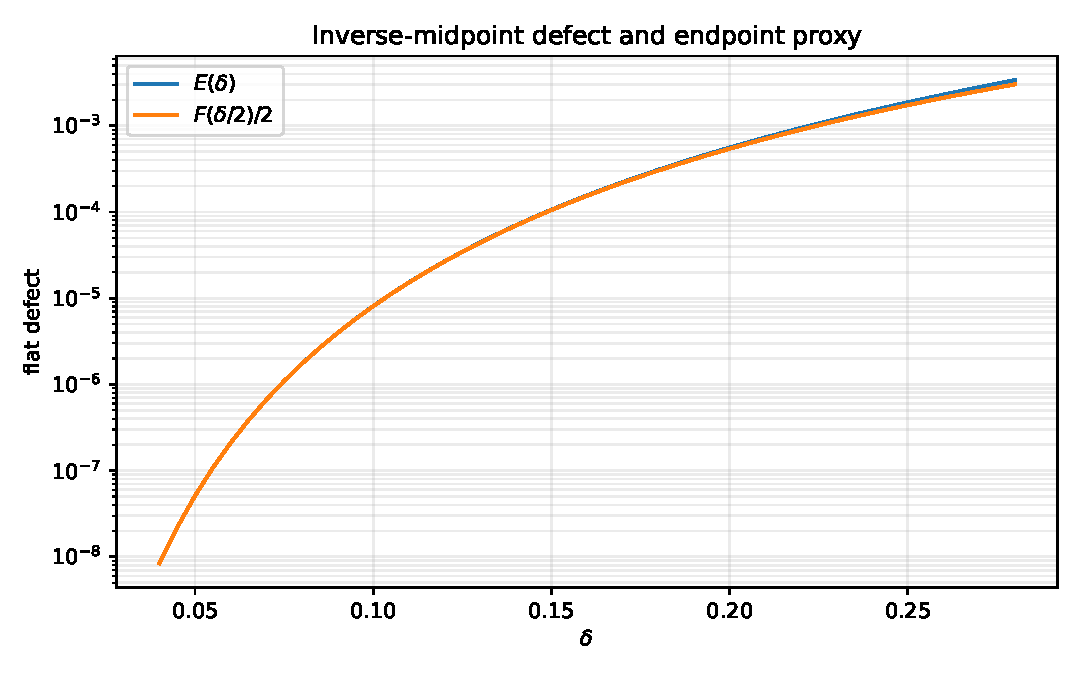
\includegraphics[width=0.92\textwidth]{figures/inverse_midpoint_defect.pdf}
\caption{The exact inverse midpoint defect $E(\delta)$ and the leading endpoint proxy $F(\delta/2)/2$.  Their relative separation rapidly becomes invisible on the logarithmic vertical scale, in agreement with \cref{prop:inverse-proxy}.}
\label{fig:inverse-defect}
\end{figure}

\subsection{Exact dyadic arithmetic}
The code reproduces, using exact fractions,
\begin{align*}
 F(1)&=1,&
 F\!\left(\frac12\right)&=\frac12,&
 F\!\left(\frac14\right)&=\frac5{72},\\
 F\!\left(\frac18\right)&=\frac1{288},&
 F\!\left(\frac1{16}\right)&=\frac{143}{2073600},&
 F\!\left(\frac1{32}\right)&=\frac{19}{33177600},\\
 F\!\left(\frac1{64}\right)&=\frac{1153}{561842749440}.&&
\end{align*}
These values are not new; they serve as independent regression tests for the numerical evaluator and establish compatibility with the repository's exact arithmetic.

\subsection{Cardinal and q-scale checks}
All q-binomial closures \eqref{eq:q-closure} through degree twelve simplified identically to zero.  For the cardinal identities, the maximum residual over the five nonlattice points
$-0.83,-0.41,0.07,0.37,0.79$ is summarized in \cref{tab:reproduction-errors}.

\begin{table}[H]
\centering
\caption{Largest numerical residual in \eqref{eq:appell-reproduction} at each tested scale.  The final column reports the hardest case $n=r$.}
\label{tab:reproduction-errors}
\begin{tabular}{@{}rrr@{}}
\toprule
$r$ & degrees tested & maximum residual\\
\midrule
0 & $0$ & $7.25\times10^{-71}$\\
1 & $0,1$ & $4.52\times10^{-20}$\\
2 & $0,1,2$ & $2.36\times10^{-19}$\\
3 & $0,1,2,3$ & $4.72\times10^{-18}$\\
4 & $0,1,2,3,4$ & $5.67\times10^{-17}$\\
5 & $0,1,2,3,4,5$ & $5.23\times10^{-14}$\\
\bottomrule
\end{tabular}
\end{table}
The growth in the last row is expected from cancellation between large polynomial samples and does not indicate failure of the exact identity.  Increasing the Fourier truncation reduces the approximation error; interval arithmetic would instead provide a certified enclosure.

\section{A formalization roadmap}
\label{sec:formalization}

The deductions split naturally into algebraic, analytic, and special-function layers.

\subsection{Low-cost Lean targets}
The following results require only the already formalized Fabius equations, elementary integration, and inverse monotonicity:
\begin{enumerate}
\item \cref{thm:midpoint-transmutation} and the all-orders derivative statement \cref{cor:midpoint-jet};
\item the inverse fixed-point equation \eqref{eq:inverse-fixed-point};
\item flatness of $E$ from endpoint flatness and $h\sim\delta/2$;
\item monotone lower and upper fixed-point iterations from \cref{prop:certified-iteration}.
\end{enumerate}
A practical theorem statement should avoid asymptotic notation initially and prove, for every $N$, a neighborhood estimate $|E(\delta)|\le C_N|\delta|^N$.

\subsection{Finite combinatorial and algebraic targets}
The distributional identity \eqref{eq:tm-derivative} can be formalized first as a finite signed-measure convolution identity.  Its coefficient and location maps are binary sums, and the sign is exactly the existing signed Thue--Morse sequence.  The q-closure \eqref{eq:q-closure} reduces to the finite q-binomial theorem and polynomial degree bounds.  The Bernoulli transport recurrence is a formal power-series coefficient calculation and is likewise independent of analytic convergence.

\subsection{Fourier and periodization targets}
A formal proof of \cref{thm:moment-periodization} needs:
\begin{itemize}
\item Fourier transforms of compactly supported smooth functions;
\item differentiation under the integral;
\item periodization and Fourier coefficients;
\item the zero multiplicity of a finite or infinite sinc product.
\end{itemize}
A staged approach can first prove the identities for finite box convolutions, where all transforms are finite products, and then pass to $U_r$ by the existing approximation limits.

\subsection{Holonomic infrastructure}
The D-finite results require a library definition of polynomial-coefficient linear differential equations and the ordinary-point analyticity/uniqueness theorem.  Once that infrastructure exists, both obstructions are short:
\begin{itemize}
\item dense dyadic nonanalyticity contradicts ordinary-point analyticity;
\item a zero of multiplicity at least the equation order at an ordinary point contradicts uniqueness.
\end{itemize}
The P-recursive corollaries then require the standard equivalence between recurrences and D-finite generating functions.

\section{Further frontier problems}
\label{sec:open}

\begin{frontieropenbox}[title=1. Differential transcendence]
Non-D-finiteness excludes linear polynomial-coefficient differential equations but not nonlinear algebraic differential equations.  Determine whether $F$, $I$, $U$, $\widehat U$, or $\M_0$ is differentially algebraic over $\C(x)$.  The infinite hierarchy of zero multiplicities and the dilation functional equations may provide a route to differential transcendence.
\end{frontieropenbox}

\begin{frontieropenbox}[title=2. Convergence and resurgence of the inverse Lagrange--Bell coupling series]
The finite jet \eqref{eq:lagrange-finite} is rigorous, but convergence of the full series at $\varepsilon=1$ is not asserted.  Estimate the growth of
$\D^{n-1}[F(z)^n]$ uniformly as $z\downarrow0$, identify a possible Gevrey order, and test Borel summability.  The lower-Lambert coordinate should separate algebraic saddle corrections from the flat fixed-point feedback.
\end{frontieropenbox}

\begin{frontieropenbox}[title=3. Exact two-adic denominator laws for the cardinal Appell family]
The coefficients in \eqref{eq:first-appell-polys} combine Bernoulli denominators with the factors $2^{2m}-1$.  Determine exact $2$-adic and odd-prime valuations of the coefficients of $\Acard_n(x;Q)$, and compare them with the denominator phenomena in the repository's exact dyadic Fabius values.
\end{frontieropenbox}

\begin{frontieropenbox}[title=4. Stability of coarsening reproduction]
The identities \eqref{eq:appell-reproduction} are exact, but the sampling coefficients grow with $r$ and $n$.  Determine the optimal condition numbers, Lebesgue-type constants, and noise amplification of the finite cardinal sums.  Seek dual kernels or mixed scales that preserve exactness while controlling cancellation.
\end{frontieropenbox}

\begin{frontieropenbox}[title=5. Base-$b$ Prouhet kernels]
Replace the dyadic random series by uniform digits in base $b$ and the Thue--Morse sign by a root-of-unity digit character.  The finite block should produce a Prouhet cancellation of prescribed order, while the infinite tail produces a $b$-adic zero-multiplicity correction.  Develop the analogue of the Appell ladder and identify its q-scale closure at $q=b^{-2}$.
\end{frontieropenbox}

\begin{frontieropenbox}[title=6. q-holonomic versus P-recursive scale sequences]
For fixed $n$, the scale sequence $r\mapsto\Acard_n^{[r]}(x)$ satisfies a finite q-binomial closure because it is a polynomial in $4^r$.  For fixed $r$, the degree sequence $n\mapsto\Acard_n^{[r]}(x)$ is not P-recursive.  This sharp asymmetry suggests studying whether it is q-holonomic in $n$, or whether the infinite pole lattice also rules out natural q-difference classes.
\end{frontieropenbox}

\begin{frontieropenbox}[title=7. Phase-resolved inverse extrapolation]
Equation \eqref{eq:inverse-lambert-transfer} says that the inverse midpoint defect inherits the endpoint periodic phase exactly.  Construct phase-locked Richardson schemes directly for $I(1/2+\delta)$, and compare them with schemes that first approximate $F$ and then invert.  The fixed-point enclosure supplies rigorous error certificates.
\end{frontieropenbox}

\begin{frontieropenbox}[title=8. Multivariate pseudo-box analogues]
The approximation literature contains multivariate pseudo-box splines and nonstationary refinable systems.  Determine which products possess a valuation-indexed zero multiplicity strong enough to create an increasing cardinal reproduction ladder, and whether multivariate Prouhet arrays replace the finite Thue--Morse block in \eqref{eq:tm-derivative}.
\end{frontieropenbox}

\section{Conclusion}
The corpus already explains why q-binomial coefficients, infinite sinc products, Lambert--W functions, Bell polynomials, Lagrange interpolation, and Richardson extrapolation occur around the Fabius and Rvachev functions.  The present report adds three cross-connections.

The midpoint is not merely symmetric: after subtracting its affine tangent, it is exactly the negative of the endpoint function.  This identity upgrades the known first two inverse derivatives to an all-orders flatness theorem, furnishes a certified fixed-point inverse, and transports the complete endpoint Lambert--W expansion to the inverse midpoint defect.

The integer zeros of the Fourier transform are not merely spectral curiosities: under dyadic dilation, their multiplicities form a Strang--Fix ladder.  A finite Prouhet--Thue--Morse block supplies the universal order, moment periodization supplies exact cardinal identities, reciprocal moments supply Appell correctors, Bernoulli cumulants and Bell polynomials supply their coefficients, and Gaussian binomials supply exact scale closures.

Finally, the same dyadic structure obstructs holonomicity in two directions.  In physical space it produces dense nonanalyticity; in Fourier space it produces zeros of unbounded multiplicity.  The consequences extend from $F$, $F^{-1}$, and $\Up$ to their moment and Appell sequences.  These deductions are compact enough to be plausible formalization targets, yet broad enough to open new research programs in differential algebra, exact sampling, q-holonomicity, and base-$b$ generalization.

\appendix

\section{Additional proof details}
\label{app:proof-details}

\subsection{Barycentric denominator calculation}
For completeness, let $0\le j\le d$.  Split the denominator into indices below and above $j$:
\begin{align*}
 \prod_{\ell\ne j}(q^{-j}-q^{-\ell})
 &=\left[\prod_{\ell=0}^{j-1}q^{-j}(1-q^{j-\ell})\right]
   \left[\prod_{\ell=j+1}^{d}-q^{-\ell}(1-q^{\ell-j})\right]\\
 &=(-1)^{d-j}q^{-\binom{d+1}{2}-\binom j2}
   (q;q)_j(q;q)_{d-j}.
\end{align*}
Taking the reciprocal gives \eqref{eq:barycentric-q}.

\subsection{Why the inverse correction is beyond every Lambert order}
From $h\sim z$ and endpoint flatness, $F'(h)=2F(2h)$ is smaller than every power of $h$.  The lower-Lambert relation $z=\lambda2^{-\lambda}$ implies
$z^a=\lambda^a\e^{-aL\lambda}$, which is itself smaller than every power $\lambda^{-N}$.  Therefore
\[
 F'(h)=\bigO(z^a)=\smallo(\lambda^{-N})
\]
for arbitrary $a,N>0$, proving that the logarithmic correction in \eqref{eq:log-proxy} cannot alter any coefficient in the algebraic $1/\lambda$ expansion.

\subsection{Ordinary-point analyticity}
If $p_m(x_0)\ne0$ in \eqref{eq:Dfinite}, divide by $p_m$ to obtain an analytic first-order system for the vector
$(y,y',\ldots,y^{(m-1)})$.  Standard existence and uniqueness produce a convergent power series solution for any initial vector.  Hence every $C^m$ solution of the equation is analytic near $x_0$.  This is the only differential-equation fact needed in \cref{thm:physical-nondfinite,thm:fourier-nondfinite}.

\section{Explicit Appell polynomials through degree eight}
\label{app:polynomials}
Put $Q=4^r$.  In addition to \eqref{eq:first-appell-polys},
\begin{align*}
 \Acard_7(x;Q)
 &=x^7-\frac73Qx^5+\frac{217}{135}Q^2x^3
   -\frac{2347}{8505}Q^3x,\\[0.4em]
 \Acard_8(x;Q)
 &=x^8-\frac{28}{9}Qx^6+\frac{434}{135}Q^2x^4
   -\frac{9388}{8505}Q^3x^2
   +\frac{1904369}{32531625}Q^4.
\end{align*}
The unreduced exact forms emitted by SymPy are
\begin{align*}
 \Acard_6(x;Q)
 &=\frac{-2347Q^3+41013Q^2x^2-99225Qx^4+59535x^6}{59535},\\
 \Acard_7(x;Q)
 &=\frac{x(-2347Q^3+13671Q^2x^2-19845Qx^4+8505x^6)}{8505},\\
 \Acard_8(x;Q)
 &=\frac{1904369Q^4-35909100Q^3x^2+104583150Q^2x^4}{32531625}\\
 &\quad+\frac{-101209500Qx^6+32531625x^8}{32531625}.
\end{align*}

\section{Reproducibility files}
\label{app:reproducibility}
The ZIP archive contains:
\begin{center}
\begin{tabularx}{0.96\textwidth}{@{}>{\footnotesize\ttfamily\raggedright\arraybackslash}p{0.38\textwidth}X@{}}
\toprule
fabius\_frontier\_report.tex & Complete report source.\\
fabius\_frontier\_report.pdf & Compiled and visually inspected report.\\
frontier\_experiments.py & Fully commented symbolic/numerical program.\\
corpus\_manifest.txt & Recursive list of all fifty-seven audited TeX paths and the exclusion-search protocol.\\
results/numerical\_results.txt & Human-readable ledger of parameters and outputs.\\
results/inverse\_defect.csv & Machine-readable inverse-defect table.\\
results/reproduction\_errors.csv & Machine-readable cardinal residual table.\\
figures/*.png, figures/*.pdf & Source figures in raster and vector form.\\
README.txt & Build and rerun instructions.\\
\bottomrule
\end{tabularx}
\end{center}
The program can be rerun with
\begin{lstlisting}[style=code,language=bash]
python frontier_experiments.py
\end{lstlisting}
and the report can be rebuilt with
\begin{lstlisting}[style=code,language=bash]
latexmk -pdf -interaction=nonstopmode -halt-on-error fabius_frontier_report.tex
\end{lstlisting}

\section{Complete recursive TeX manifest}
\label{app:manifest}
\lstinputlisting[style=manifest]{corpus_manifest.txt}

\begin{thebibliography}{99}

\bibitem{proveit}
V. Reshetnikov,
\emph{ProveIt: Analysis/FabiusFunction}, GitHub repository,
\url{https://github.com/VladimirReshetnikov/ProveIt/tree/main/Analysis/FabiusFunction},
repository snapshot audited 27 August 2026.

\bibitem{primary}
V. Reshetnikov,
\emph{The Fabius Function and Rvachev's Up-Function: Exact arithmetic, probability, Fourier analysis, and corrected sharp asymptotics},
\path{Analysis/FabiusFunction/docs/Fabius_Function_and_Rvachev_Up/Fabius_Function_and_Rvachev_Up.tex}, 2026.

\bibitem{frontier}
V. Reshetnikov,
\emph{Non-formalized research frontiers for the Fabius function and Rvachev's up-function},
\path{Analysis/FabiusFunction/docs/non-formalized-research-frontiers/non-formalized-research-frontiers.tex}, 2026.

\bibitem{atlas}
V. Reshetnikov,
\emph{Thue--Morse Formula Atlas},
\path{Analysis/FabiusFunction/docs/non-formalized-research-frontiers/drafts/Thue_Morse_Formula_Atlas/Thue_Morse_Formula_Atlas.tex}, 2026.

\bibitem{ariasUp}
J. Arias de Reyna,
\emph{An infinitely differentiable function with compact support: Definition and properties},
arXiv:1702.05442, 2017.

\bibitem{ariasArithmetic}
J. Arias de Reyna,
\emph{Arithmetic of the Fabius function},
arXiv:1702.06487, 2017.

\bibitem{dynRon}
N. Dyn and A. Ron,
\emph{Multiresolution analysis by infinitely differentiable compactly supported functions},
Applied and Computational Harmonic Analysis \textbf{2} (1995), 15--20.

\bibitem{strangFix}
G. Strang and G. Fix,
\emph{A Fourier analysis of the finite element variational method},
in \emph{Constructive Aspects of Functional Analysis}, Edizioni Cremonese, Rome, 1973, 795--840.

\bibitem{liShen}
S. Li and Y. Shen,
\emph{Pseudo box splines},
Applied and Computational Harmonic Analysis \textbf{26} (2009), 344--356,
DOI: 10.1016/j.acha.2008.07.004.

\bibitem{stanley}
R. P. Stanley,
\emph{Differentiably finite power series},
European Journal of Combinatorics \textbf{1} (1980), 175--188.

\bibitem{corless}
R. M. Corless, G. H. Gonnet, D. E. G. Hare, D. J. Jeffrey, and D. E. Knuth,
\emph{On the Lambert W function},
Advances in Computational Mathematics \textbf{5} (1996), 329--359.

\bibitem{roman}
S. Roman,
\emph{The Umbral Calculus},
Academic Press, 1984.

\bibitem{comtet}
L. Comtet,
\emph{Advanced Combinatorics: The Art of Finite and Infinite Expansions},
Reidel, 1974.

\bibitem{alloucheShallit}
J.-P. Allouche and J. Shallit,
\emph{Automatic Sequences: Theory, Applications, Generalizations},
Cambridge University Press, 2003.

\bibitem{prouhet}
E. Prouhet,
\emph{Memoire sur quelques relations entre les puissances des nombres},
C. R. Acad. Sci. Paris \textbf{33} (1851), 225.

\end{thebibliography}

\end{document}
